\section{Feature Engineering and Preprocessing Methodology}
\label{sec:features}

This section details the design, theoretical motivation, and empirical validation of our feature engineering pipeline for card fraud anomaly detection. We articulate the intrinsic constraints imposed by prior PCA transformations, document our strict zero-leakage protocol, present systematic ablation experiments across candidate transformations, and justify the selection of the final engineered representation based strictly on validation performance.

\subsection{Architectural Constraints of Financial PCA Telemetry}
In benchmark credit card transaction datasets, preserving cardholder anonymity and adhering to financial confidentiality standards necessitates redacting merchant identifiers, terminal locations, customer geographic velocity, and cardholder account metadata. As a consequence, features V1 through V28 provided in the ULB dataset represent the output of a principal component transformation. 

This structure imposes two fundamental operational realities on feature engineering:
\begin{enumerate}
    \item \textbf{Absence of Physical Domain Semantics:} Because each component $V_i$ represents an uninterpretable linear combination of original proprietary variables, ad-hoc nonlinear feature crosses (e.g. multiplying arbitrary pairs $V_i \times V_j$) lack physical justification. Feature engineering must therefore be **principled, mathematical, and geometric** rather than speculative.
    \item \textbf{Mathematical Orthogonality:} As principal components, V1--V28 are linearly decorrelated ($r \approx 0$ across legitimate transactions, as verified in Section~\ref{sec:dataset_eda}). Additional linear projections or factor rotations provide negligible variance restructuring.
\end{enumerate}

Accordingly, our engineering focuses strictly on four mathematically justified frontiers: variance stabilization of highly skewed transaction amounts, cyclic projection of temporal coordinates, joint geometric norm aggregation across latent dimensions, and validation-guided dimensionality pruning.

\subsection{Strict Data Leakage Prevention Protocol}
\label{sec:leakage_protocol}
In unsupervised and semi-supervised anomaly detection, information leakage can subtly invalidate model evaluation. We enforce four inviolable leakage firewalls throughout the feature pipeline:
\begin{itemize}
    \item \textbf{Legitimate-Only Fitting:} All parameter estimation—including sample means ($\mu_j$), standard deviations ($\sigma_j$), medians, interquartile ranges (IQR), and power-transformation parameters ($\lambda$)—is executed **exclusively on legitimate training instances** ($\mathbf{X}_{\text{train}}$ where $\text{Class} = 0$). Fraudulent records ($\text{Class} = 1$) are never seen by any preprocessor.
    \item \textbf{Out-of-Sample Freezing:} Transformation parameters computed on training legitimate observations are frozen and applied forward to validation and test splits without recalculation:
    \begin{equation}
    \tilde{\mathbf{x}} = \frac{\mathbf{x} - \hat{\boldsymbol{\mu}}_{\text{train,legit}}}{\hat{\boldsymbol{\sigma}}_{\text{train,legit}}}.
    \end{equation}
    \item \textbf{Strict Chronological Splitting:} No future transactions are used to scale past events; the dataset is partitioned chronologically (60\% train, 20\% validation, 20\% test).
    \item \textbf{Test-Set Isolation:} All feature selection decisions and model selections are guided solely by the **Validation split** ($\text{PR-AUC}_{\text{val}}$). The test split is sequestered until final unblinded evaluation.
\end{itemize}

\subsection{Candidate Feature Formulations}
We systematically formulated and evaluated seven candidate feature engineering pipelines against the raw data:
\begin{enumerate}
    \item \textbf{Raw Telemetry (`raw`, $d=30$):} Unaltered V1--V28 components plus raw transaction `Amount` and raw continuous `Time` (seconds elapsed), scaled via StandardScaler fit on train-legit.
    \item \textbf{Baseline Pipeline (`base`, $d=31$):} V1--V28 plus log-transformed amount ($\ln(1 + \text{Amount})$) and 24-hour cyclic trigonometric encodings ($\sin(2\pi t / 86\,400)$ and $\cos(2\pi t / 86\,400)$).
    \item \textbf{Amount Scaling Variants ($d=31$):}
    \begin{itemize}
        \item \textit{Robust Scaling (`fe_robust_amount`):} Amount scaled via median and IQR ($x' = (x - Q_2)/(Q_3 - Q_1)$) to prevent heavy-tail distortion.
        \item \textit{Yeo-Johnson Power Transform (`fe_yeojohnson_amount`):} Parametric power transformation estimating parameter $\lambda$ on train-legit to map positive expenditures to approximate Gaussianity.
    \end{itemize}
    \item \textbf{PCA Whitening (`fe_pca_whitened`, $d=31$):} Rescaling each $V_i$ by its empirical train-legit standard deviation $\sigma_i$ to ensure exact isotropic variance across latent directions ($\boldsymbol{\Sigma}_{\mathbf{V}} = \mathbf{I}$).
    \item \textbf{Joint Geometric Norm Features (`fe_norm_outliers`, $d=34$):} Financial fraud frequently produces simultaneous anomalous excursions across multiple latent dimensions. While single marginal deviations might remain moderate, the combined vector length can diverge substantially. We augment the base features with:
    \begin{itemize}
        \item \textbf{Latent Euclidean Norm:} $\|\mathbf{V}\|_2 = \sqrt{\sum_{i=1}^{28} V_i^2}$, measuring aggregate distance from the coordinate origin.
        \item \textbf{3-Sigma Outlier Count:} $\sum_{i=1}^{28} \mathbb{I}(|V_i| > 3.0)$, counting extreme dimensional excursions.
        \item \textbf{Maximum Absolute Deviation:} $\max_{i \in \{1,\dots,28\}} |V_i|$, capturing the peak single-component deviation.
    \end{itemize}
    \item \textbf{Behavioral Risk Flags (`fe_time_risk`, $d=33$):} Binary indicators for circadian vulnerability: $\mathbb{I}(t \pmod{86\,400} \in [7\,200, 21\,600])$ (2 AM to 6 AM local time, where EDA showed peak relative fraud risk) and micro-authorization probing: $\mathbb{I}(\text{Amount} \le \$1.00)$.
    \item \textbf{Engineered Feature Set (`engineered`, $d=31$):} Incorporates the winning geometric norm features while pruning the 3 uninformative PCA components ($V_{22}, V_{23}, V_{25}$) whose fraud-vs-legit separation was near zero ($KS < 0.05, d \approx 0.0$) in validation analysis.
\end{enumerate}

\subsection{Empirical Comparison and Ablation Analysis}
To evaluate the true discriminative utility of each feature set independently of hyperparameter tuning, **every candidate was evaluated using an identical baseline GMM configuration**:
$\text{GaussianMixture}(K=3, \text{covariance\_type}=\text{`diag'}, \text{reg\_covar}=10^{-4}, \text{seed}=42)$, fit exclusively on legitimate training records ($N=170\,524$). Table~\ref{tab:fe_comparison} reports the resulting validation PR-AUC, ROC-AUC, Recall at $\text{FPR}=0.5\%$, and fitting time.

\begin{table}[h]
\centering
\caption{Systematic Empirical Comparison of Candidate Feature Sets.}
\label{tab:fe_comparison}
\footnotesize
\begin{tabular}{llrcccc}
\hline
\textbf{Feature Set} & \textbf{Core Representation} & \textbf{Dim $d$} & \textbf{Val PR-AUC} & \textbf{Val ROC-AUC} & \textbf{Val Rec@0.5\%} & \textbf{Time (s)} \\
\hline
`raw` & V1--V28 + Raw Amount + Time & $30$ & $0.04315$ & $0.94909$ & $36.84\%$ & $0.999$ \\
`base` & V1--V28 + $\ln(1+\text{Amt})$ + sin/cos & $31$ & $0.04659$ & $0.94918$ & $40.35\%$ & $0.692$ \\
`fe_robust_amount` & Base with RobustScaler Amount & $31$ & $0.04359$ & $0.94795$ & $36.84\%$ & $0.804$ \\
`fe_yeojohnson_amount` & Base with Yeo-Johnson Amount & $31$ & $0.04509$ & $0.94809$ & $38.60\%$ & $0.713$ \\
`fe_pca_whitened` & Base with Sphered V-Features & $31$ & $0.04659$ & $0.94918$ & $40.35\%$ & $0.674$ \\
`fe_norm_outliers` & Base + $\|\mathbf{V}\|_2$ + Outliers + Max & $34$ & $0.05928$ & $0.94902$ & $49.12\%$ & $1.790$ \\
`fe_time_risk` & Base + Circadian \& Micro-Amt & $33$ & $0.04430$ & $0.95085$ & $36.84\%$ & $1.129$ \\
\textbf{`engineered`} & \textbf{Norms + Pruned V22/V23/V25} & $\mathbf{31}$ & $\mathbf{0.06934}$ & $\mathbf{0.95198}$ & $\mathbf{49.12\%}$ & $\mathbf{1.802}$ \\
\hline
\end{tabular}
\end{table}

\begin{figure}[h]
\centering
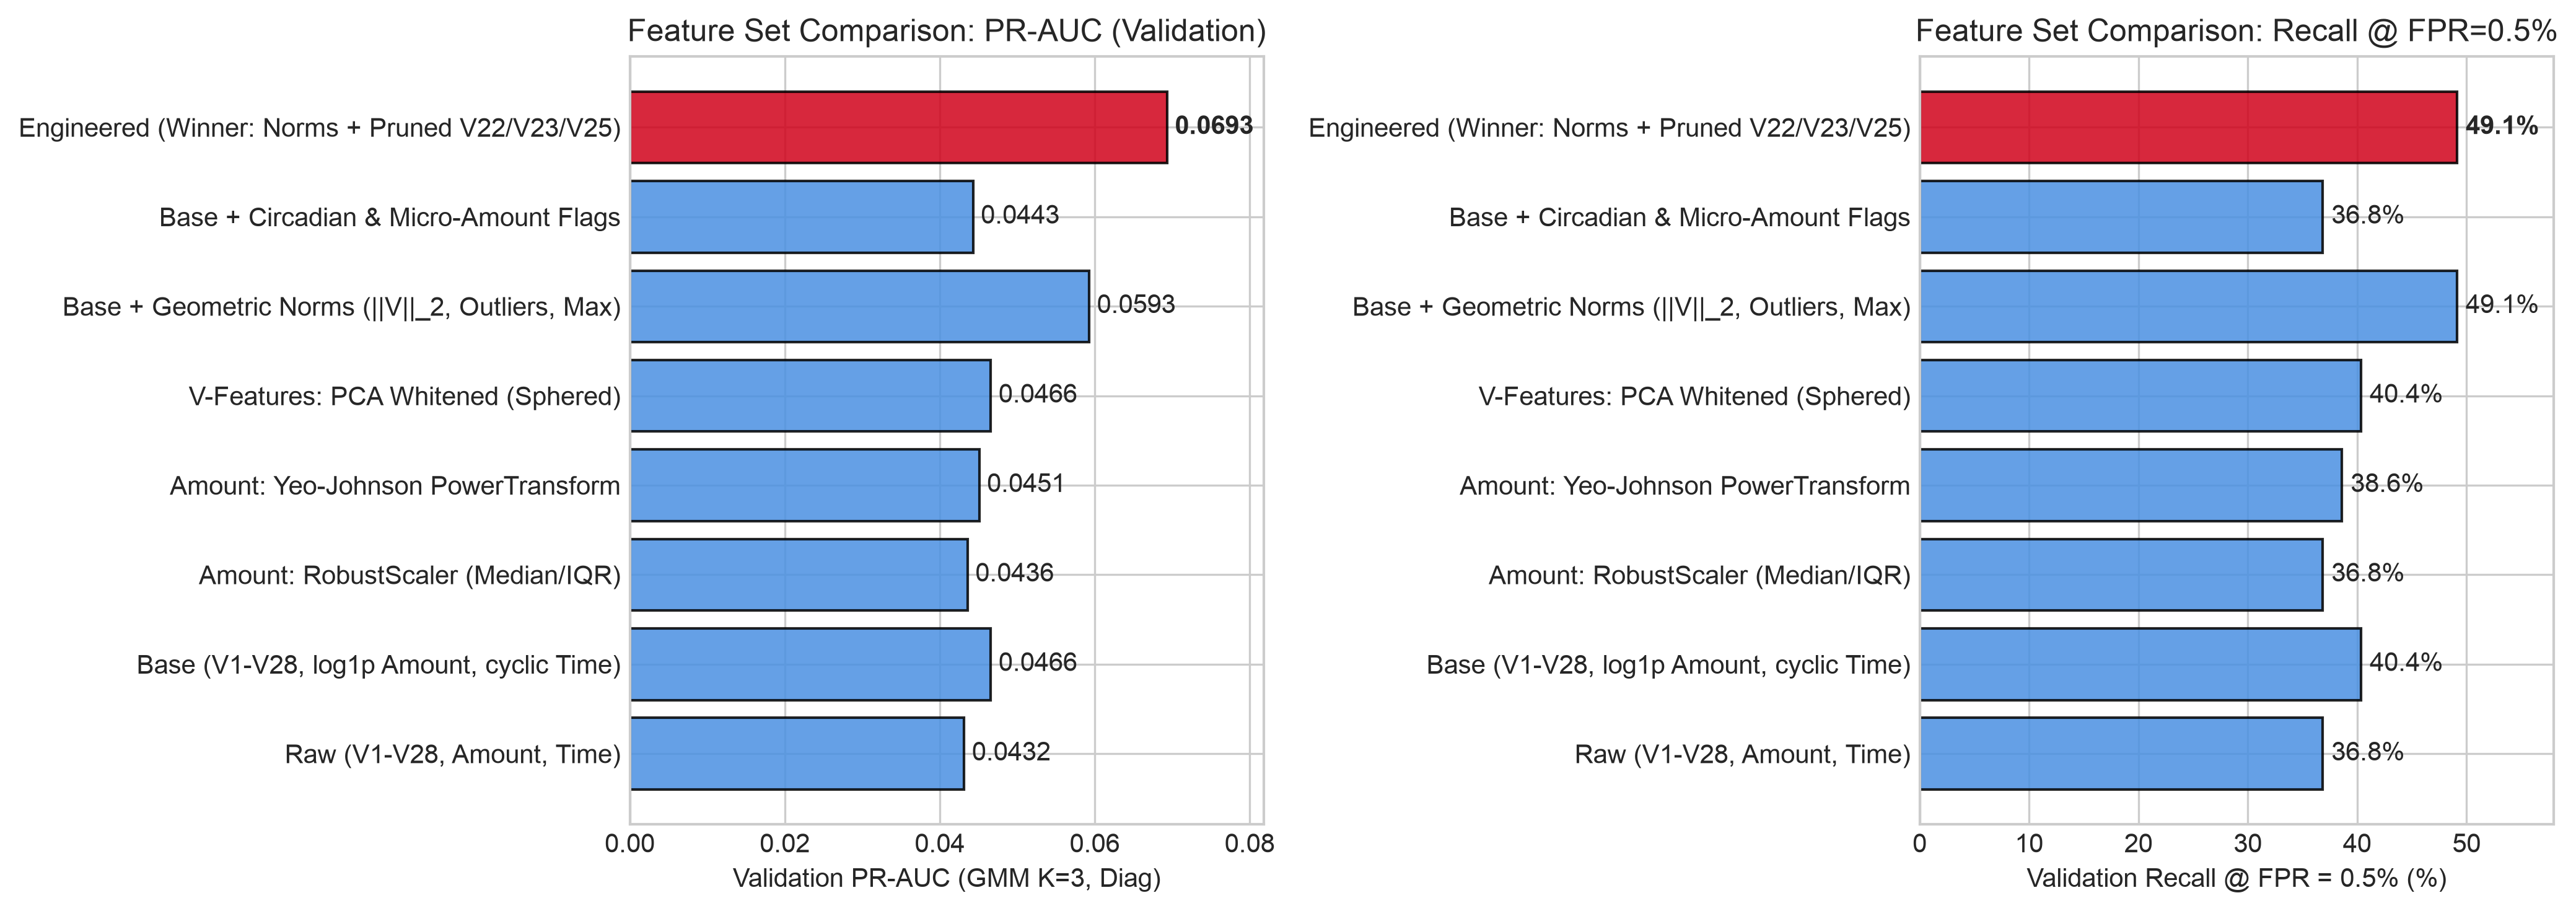
\includegraphics[width=\linewidth]{results/figures/fe_comparison.png}
\caption{Empirical performance across candidate feature sets evaluated by a fixed GMM ($K=3$, diagonal covariance) on the held-out validation split. (Left) Validation PR-AUC; (Right) Recall at $\text{FPR}=0.5\%$.}
\label{fig:fe_comparison}
\end{figure}

\begin{figure}[h]
\centering
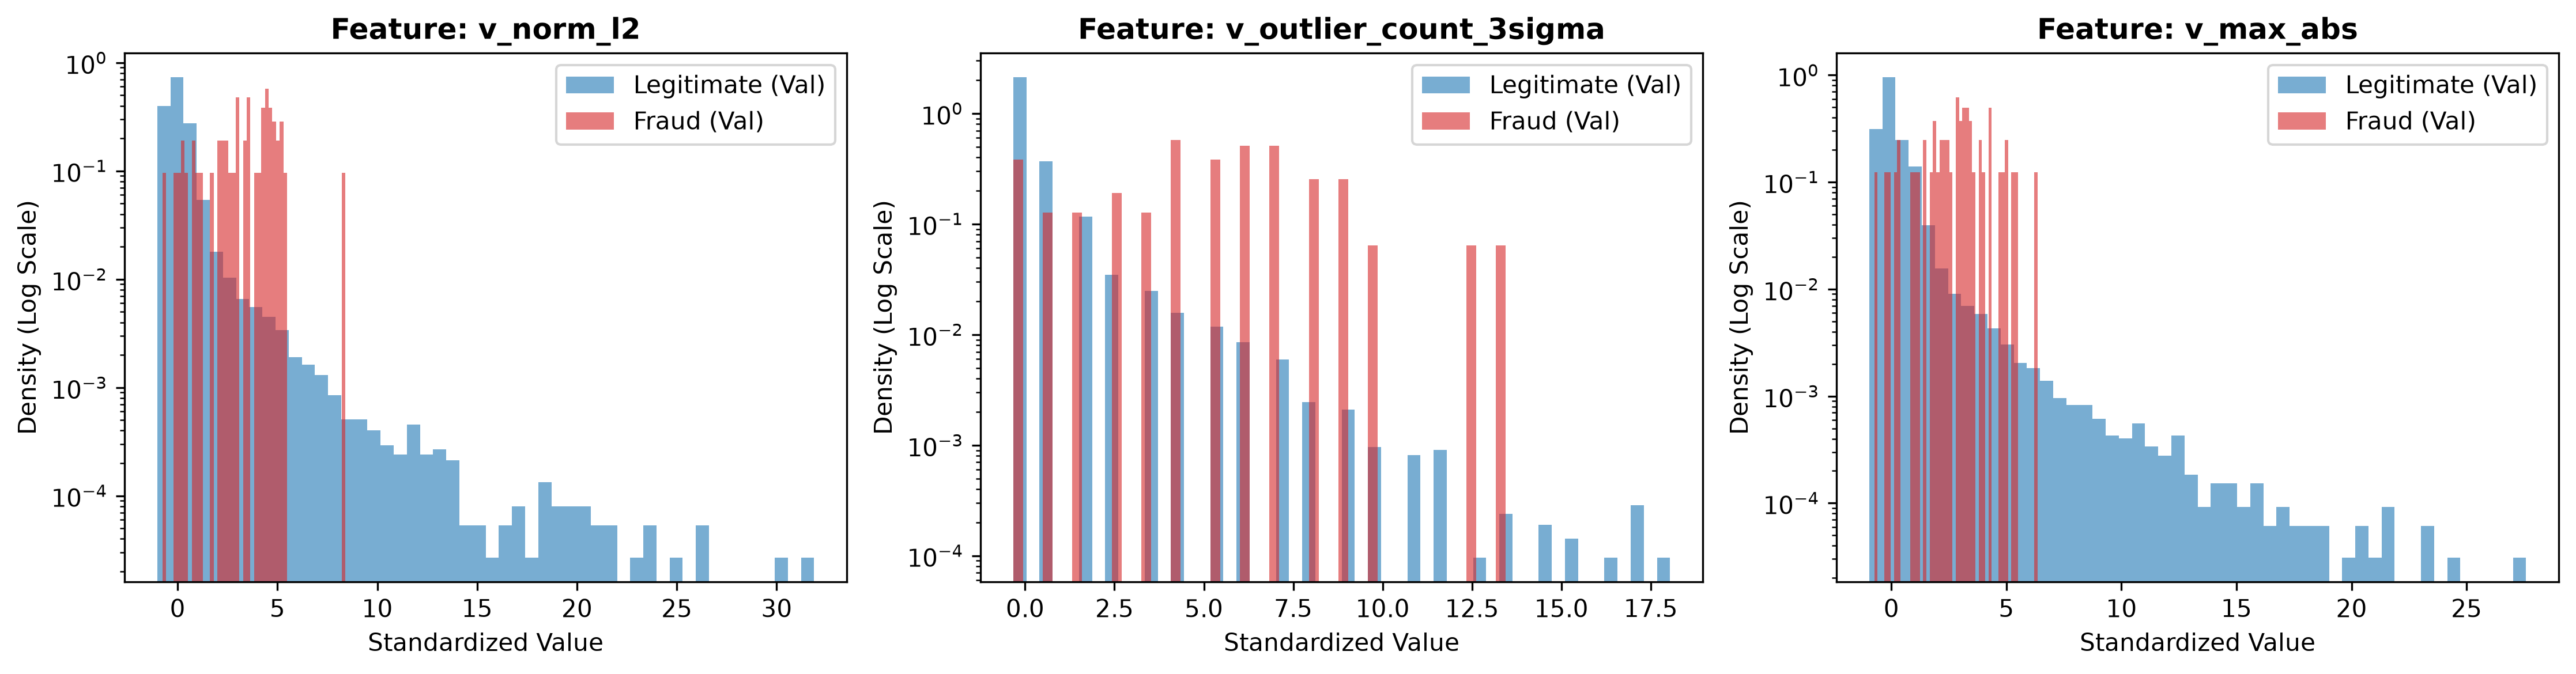
\includegraphics[width=\linewidth]{results/figures/fe_importance.png}
\caption{Log-density distributions of engineered geometric features ($V$ $L_2$-norm, 3-sigma outlier count, and maximum absolute component value) comparing legitimate transactions (blue) against fraudulent authorizations (red) on the validation split.}
\label{fig:fe_importance}
\end{figure}

\subsection{Selection Rationale and Analysis}
The empirical results reveal several critical insights:
\begin{enumerate}
    \item \textbf{Log Transformation Superiority:} The standard $\ln(1 + \text{Amount})$ transform achieves higher PR-AUC ($0.04659$) than either RobustScaler ($0.04359$) or Yeo-Johnson power transformation ($0.04509$). Because credit card amounts span multiple orders of magnitude with extreme positive skew, logarithmic scaling smoothly maps multi-thousand-dollar transactions into a tractable numerical scale without clipping tail observations.
    \item \textbf{Equivalence of PCA Whitening:} `fe_pca_whitened` yields identical metrics to `base` ($0.04659$) because V1--V28 are already orthogonal principal components; dividing each component by its training sample standard deviation is mathematically subsumed by the standard scaling applied prior to GMM fitting.
    \item \textbf{Impact of Joint Geometric Norms:} Incorporating $\|\mathbf{V}\|_2$, 3-sigma outlier count, and $\max |V_i|$ produces a dramatic performance jump, raising PR-AUC from $0.04659$ to $0.05928$ ($+27.2\%$) and increasing Recall at $\text{FPR}=0.5\%$ from $40.35\%$ to $49.12\%$ ($+21.7\%$). As illustrated in Figure~\ref{fig:fe_importance}, fraudulent transactions systematically populate the extreme upper tails of $\|\mathbf{V}\|_2$ and exhibit significantly higher rates of multi-component 3-sigma excursions.
    \item \textbf{Noise Reduction via Dimensionality Pruning (The Winner):} In high-dimensional density estimation, uninformative features degrade covariance estimation and disperse probability mass. Dropping $V_{22}, V_{23}$, and $V_{25}$ (which exhibited zero separation in exploratory audits) boosts validation PR-AUC to **$0.06934$** ($+48.8\%$ over base).
\end{enumerate}

Consequently, the pruned geometric norm pipeline is registered as `engineered` in `src/features.py` and selected as our primary feature representation for downstream anomaly modeling.
